\documentclass[hidelinks,12pt,a4paper]{article}
\usepackage[italian]{babel}
\usepackage[utf8]{inputenc}
\usepackage{fourier} 

% Images
\usepackage{graphicx}
\usepackage{caption}
\usepackage{subcaption}
\usepackage{float}
\graphicspath{ {../Images} }

% Stop hyphenation
\usepackage[none]{hyphenat}

% Dotted frame.
\usepackage{tikz}

\usepackage{changepage}

% License
\usepackage[
type={CC},
modifier={by-nc-sa},
version={4.0},
]{doclicense}

\begin{document}
	
	\title{\textbf{\centering{Laboratorio creativo per bambini}\\Collega le immagini alla descrizione}}
	\author{Alice Balestieri}
	\date{}
	
	\maketitle
	\newpage
	
	\tableofcontents
	\newpage
	
	\section{Come giocare}
	\begin{center}
		\textbf{Le regole sono rivolte agli operatori.}
	\end{center}
	
	\subsection{Variante 1}
	Una volta aver ritagliato le immagini e le descrizioni (presenti nella sezione successiva), disporle casualmente su un tavolo. I bambini dovranno riunire le immagini alla propria descrizione sovrapponendo quest'ultima all'immagine che descrive.\\
	Quando i bambini hanno finito di creare le coppie, procedere alla correzione spiegata.
	
	\subsection{Variante 2}
	Una volta aver ritagliato le immagini e le descrizioni (presenti nella sezione successiva), disporre casualmente le immagini su un tavolo e mescolare le descrizioni depositando poi il mazzo in un angolo del tavolo.\\
	 Dividere i bambini in squadre. A turno ogni squadra dovrà pescare una descrizione dal mazzo e accoppiare quest'ultima ad una immagine presente sul tavolo.\\
	Si procede subito alla correzione, se la coppia formata è corretta, la squadra trattiene le carte e termina in turno. Nel caso in cui la coppia formata non sia corretta (evitando di lasciare intendere quale possa essere la soluzione), la squadra termina il turno. L'immagine viene riposizionata sul tavolo e la descrizione viene rimescolata nel mazzo delle descrizioni.\\
	Quando le squadre dei bambini hanno finito di creare le coppie corrette, la squadra che possiede il maggior numero di carte, vince il gioco.
	
	\vspace*{\fill}
	\fboxrule=2pt
	\fbox
	{
		\begin{minipage}{\linewidth}
			In caso di dubbi per la correzione, tenere una copia digitale di questo documento consultabile dallo "smartphone". Nella sezione "Immagini e descrizioni" ogni immagine è presentata con la relativa descrizione posta inferiormente.
		\end{minipage}
	 }
	
	\newpage
	\section{Immagini e descrizioni}
%-------- Starting images & descriptions section --------
	\begin{figure}[h]
			\centering
			\begin{tikzpicture}
				\node[draw,dashed]
				{
					\fboxrule=4pt			
					\fcolorbox{white}{white}{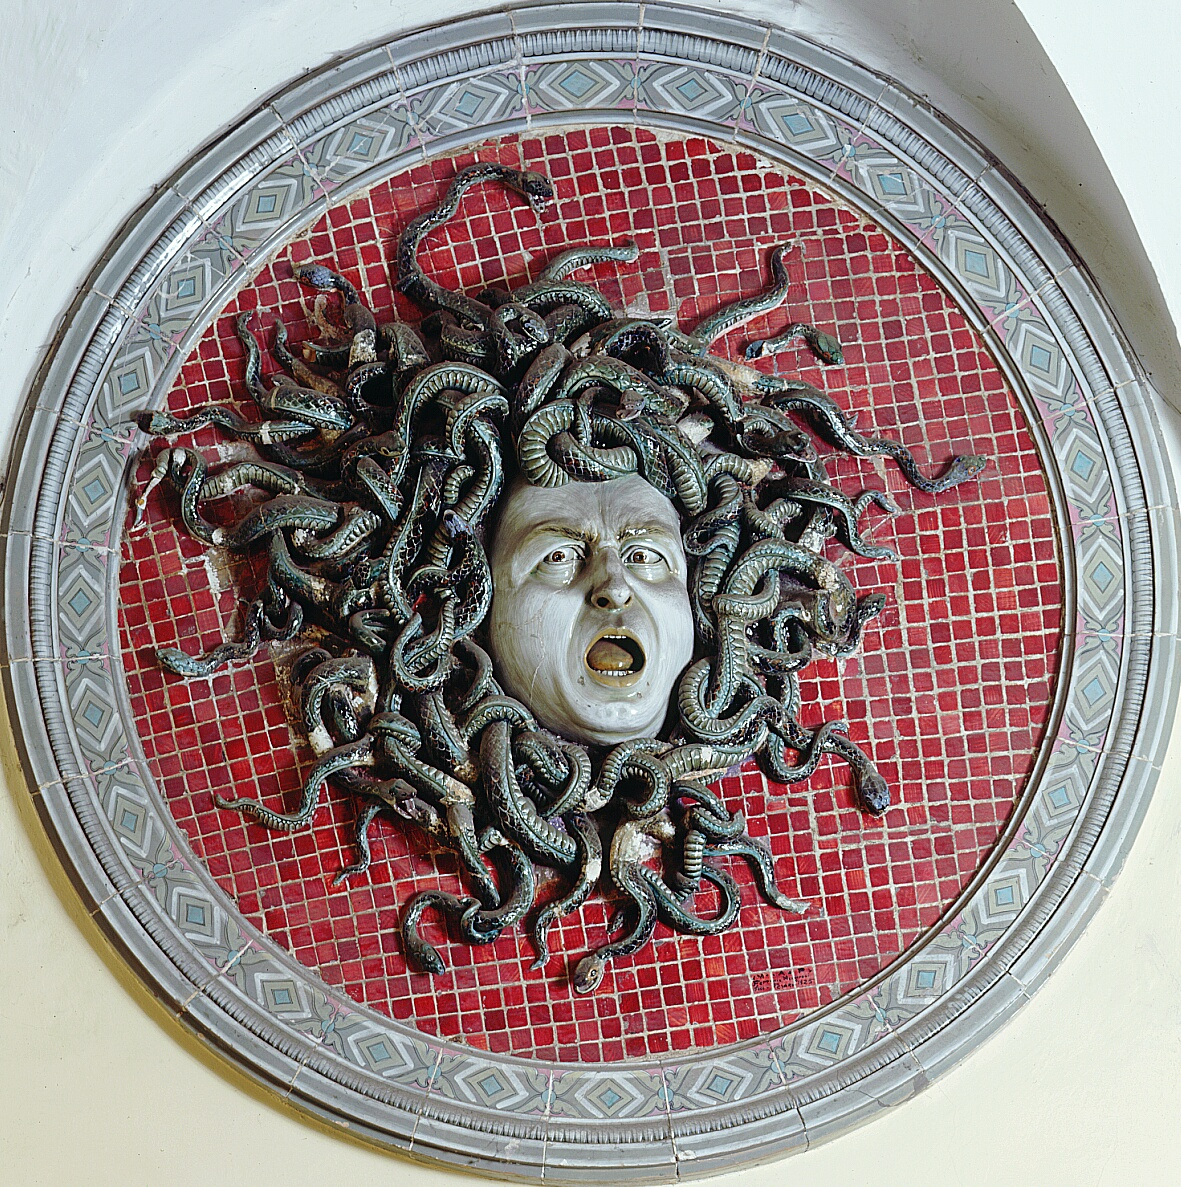
\includegraphics[scale=2]{Mengaroni_Ferruccio-Medusa.jpg}}
				};
			\end{tikzpicture}
	\end{figure}

	\begin{minipage}{\linewidth}
		\centering
		\begin{tikzpicture}
				\node[draw,dashed]
				{
					\fboxrule=4pt
					\fcolorbox{white}{white}{
						\fbox{
							\begin{minipage}{60mm}
								La testa della Medusa, circondata da molte serpi sinuose, raffigura il volto di Ferruccio Mengaroni; il fondo del tondo è a tessere rosse. Colori: verde scuro, verde ramina, bianco, mezzatinta, manganese, grigio, azzurro spento e rosa. Su quattro tessere è scritto: "M.A.P. / Ferruccio Mengaroni / fece 'Pesaro' 1925".
							\end{minipage}
						}
					}
				};
		\end{tikzpicture}
	\end{minipage}

	\newpage
	
		\begin{figure}[h]
		\centering
		\begin{tikzpicture}
			\node[draw,dashed]
			{
				\fboxrule=4pt			
				\fcolorbox{white}{white}{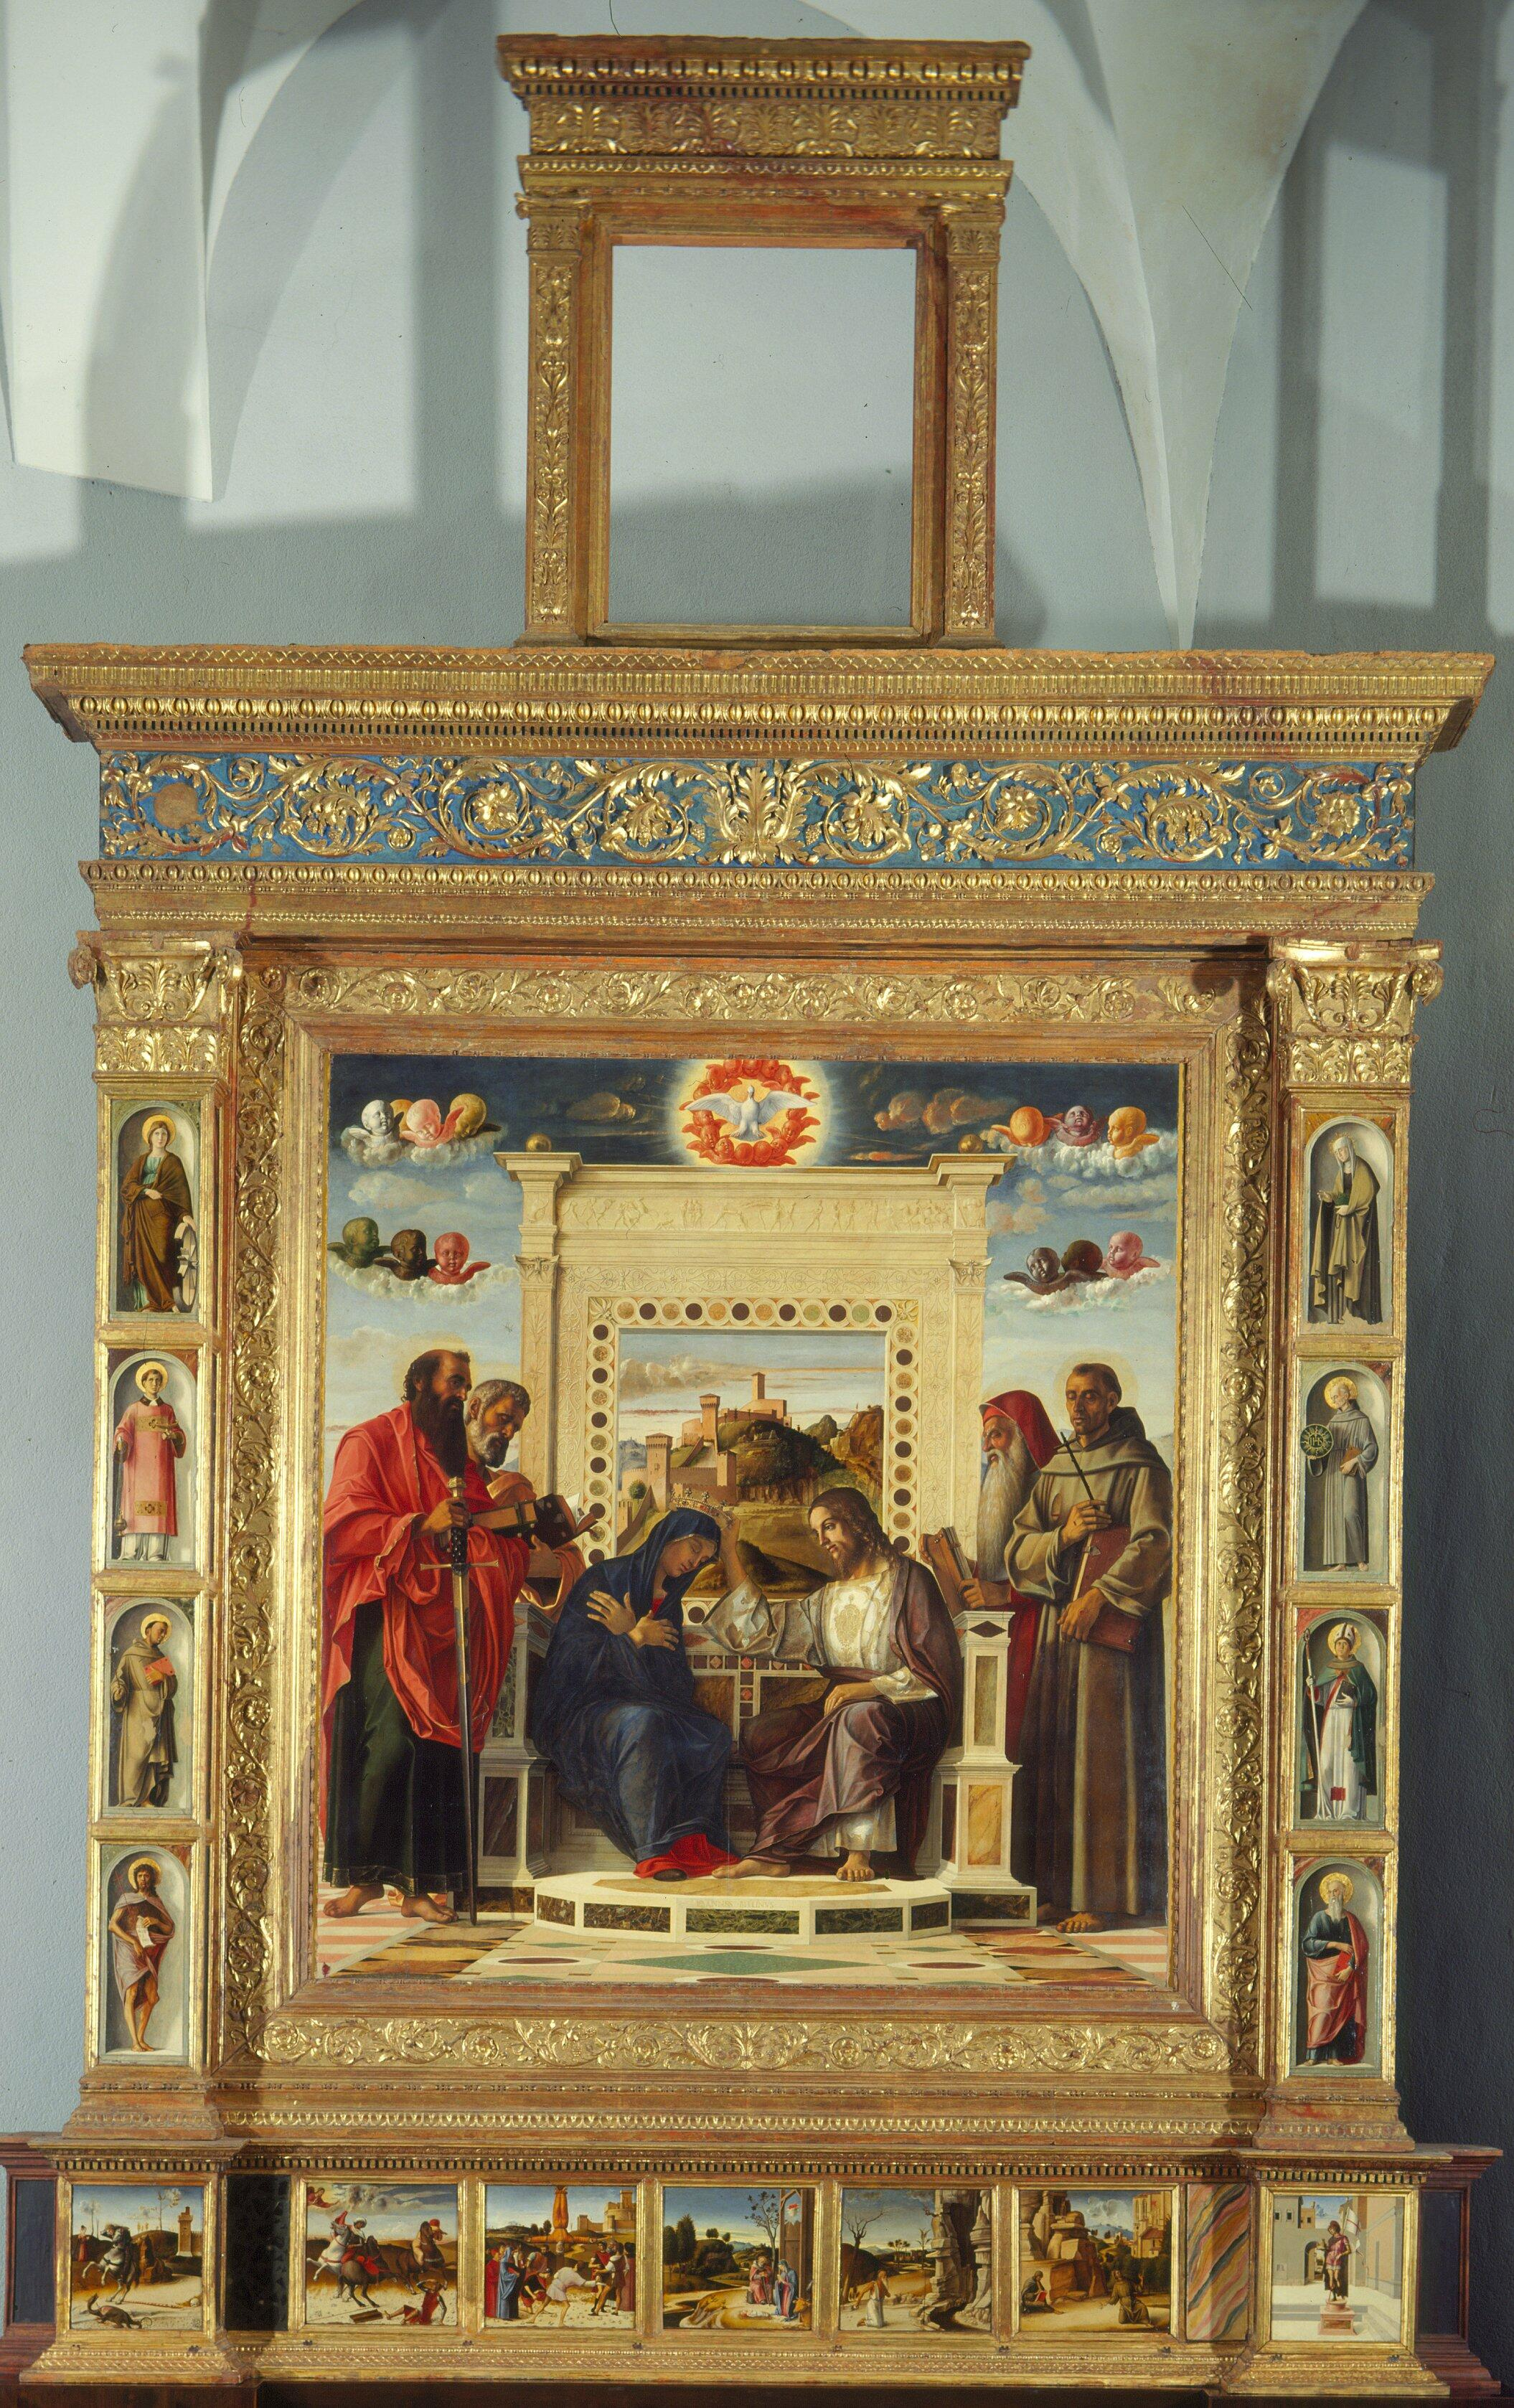
\includegraphics[scale=0.1]{Bellini_Giovanni-Incoronazione_della_Vergine.jpg}}
			};
		\end{tikzpicture}
	\end{figure}
	
	\begin{adjustwidth}{-30mm}{0mm}
		\begin{tikzpicture}
			\node[draw,dashed]
			{
				\fboxrule=4pt
				\fcolorbox{white}{white}{
					\fbox{
						\begin{minipage}{180mm}
							La pala è composta di un pannello centrale incorniciato entro un riquadro con ornati fitomorfi a girali. Sopra il pannello è collocato un architrave a girali lignei in rilievo. Di fianco sono due paraste suddivise in quattro scomparti con Santi e sormontati da due peducci. In basso la predella è divisa in cinque riquadri centrali e due ai lati. Il pannello centrale raffigura l'Incoronazione della Vergine, alla quale Cristo assiso in un trono colloca la corona sul capo. Ai lati delle due figure principali sono rappresentati in piedi i santi Paolo e Pietro, Girolamo e Francesco. Dietro Cristo e la Madonna è raffigurato un castello incorniciato dall'alzata del trono mirabilmente intarsiata e decorata a rilievi. In alto tra le nubi sono rappresentati cherubini e la colomba dello Spirito Santo. I santi rappresentati sulle paraste sono i seguenti da sinistra a destra e dall'alto in basso: la Santa Caterina, S. Lorenzo, S. Antonio da Padova, S. Giovanni Battista, la Beata Michelina, S. Bernardino da Siena, S. Ludovico da Tolosa e S. Andrea. Nella predella sono raffigurati ai lati: S. Giorgio che libera la principessa dal drago, e S. Terenzio, patrono di Pesaro; al centro S. Paolo che cade da cavallo, la Crocefissione di S. Pietro, la Natività, S. Girolamo nel deserto e S. Francesco stigmatizzato. 
						\end{minipage}
					}
				}
			};
		\end{tikzpicture}
	\end{adjustwidth}

	\newpage
		
		
	
	
\end{document}